\documentclass[12pt,oneside,slovak,a4paper]{article}

\usepackage[slovak]{babel}
\usepackage[utf8]{inputenc}
\usepackage{amsmath}
\usepackage{amsfonts}
\usepackage{amssymb}
\usepackage{graphicx}
\usepackage{cite}
\usepackage[IL2]{fontenc} % lepšia sadzba písmena Ľ než v T1
\usepackage{pdfpages}
\usepackage{url} % príkaz \url na formátovanie URL
\usepackage[hidelinks]{hyperref} % odkazy v texte budú aktívne (pri niektorých triedach dokumentov spôsobuje posun textu)
\usepackage[left=2cm,right=2cm,top=2cm,bottom=2cm]{geometry}
\usepackage{float}
\usepackage[normalem]{ulem}
\useunder{\uline}{\ul}{}
\usepackage{titling}
\usepackage{xcolor}
\usepackage{lipsum}
\usepackage{setspace}
\usepackage{blindtext}
\usepackage{caption}
\usepackage{tabularx}
\usepackage[numbers]{natbib}

% riadkovanie 1.5
\begin{document}
\linespread{1.5}\selectfont

\begin{titlepage}
	\centering
    {\Large Slovenská technická univerzita v Bratislave\par}
    {\Large Fakulta informatiky a informačných technológií\par}
	\vspace{7cm}
	{\huge\bfseries Voľne šíriteľné nástroje na obnovu zmazaných súborov\par}
	\vspace{0.5cm}
    {\Large \textsc{Princípy informačnej bezpečnosti}\par}
    \vspace{1cm}
	{\Large\itshape Marek Čederle\par}
    {\small\texttt{xcederlem@stuba.sk}\par}
	\vfill

	{\large \today\par}
\end{titlepage}


\tableofcontents
\vspace*{\fill}


\section{Špecifikácia projektu / Úvod}
V mojom projekte sa budem venovať analýze súborových systémov pre operačné systémy Windows a GNU+Linux. Bude sa jednať o súborové systémy typu NTFS a ext ale spomeniem aj dodnes veľmi používané FAT32 a exFAT ktoré sa používajú na prenosných médiách. Každý súborový systém by som chcel opísať s tým, že uvediem jeho výhody a nevýhody prípadné porovnanie s ďalšími spomenutými súborovými systémami.

Budem sa zaoberať aj tým, ako správne naformátovať disk (prepísať ho náhodnými dátami alebo samými nulami) aby pri jeho predaji sa z bezpečnostných dôvodov nedalo zistiť čo sa na ňom pred tým nachádzalo. Je to z dôvodu že pri mazaní dát z disku sa vlastne tieto dáta reálne nemažú. Dáta na disku zostanú, len sa z tabuľky záznamov zahodí záznam kde sa súbor nachádza a potom keď sa zapisuje na disk tak operačný systém vie, že môže na toto miesto zapisovať. 

Taktiež sa budem zaoberať analýzou nástroja na obnovu zmazaných súborov s názvom testdisk. Vysvetlím, prečo som si vybral práve tento nástroj. S týmto nástrojom budem následne experimentovať. Experimenty budú spočívať v tom, že si naformátujem disk a vytvorím na ňom nejaké partície podľa typu daného súborového systému. Následne naň uložím rôzne typy súborov. Budú sa tam nachádzať fotky, textové súbory, archívy, atď. Potom vymažem nejaké z týchto súborov, ale na disk ďalej nič nezapíšem, aby sa nezačali prepisovať dané miesta na disku inými súbormi. Následne vyskúšam nástroj na obnovu zmazaných súborov (testdisk) či zvládne tieto súbory obnoviť. Tento experiment zopakujem s tým, že po zmazaní ďalších súborov zapíšem na disk zase nové súbory a vyskúšam použiť nástroj na obnovu či dokáže aj po takejto akcii obnoviť súbory. Ďalší experiment bude spočívať v zmazaní celej partície a jej následnej obnove týmto nástrojom. V neposlednom rade ukážem, že po správnom formátovaní disku sa nebudú dať dáta obnoviť. Na záver budem prezentovať výsledky experimentov.
\subsection{Progress report č.1}
V prvom progress reporte vypracujem teoretickú časť, ktorú som na začiatku uviedol. To znamená popísanie rôznych typov súborových systémov a nástrojov na obnovu súborov. V neposlednom rade uvediem ako z bezpečnostného hľadiska správne ``zmazať'' súbory na disku respektíve ako ho naformátovať tak, aby sa z neho minulé dáta nedali prečítať.

\subsection{Progress report č.2}
V tomto progress reporte sa budem zameriavať na praktickú/experimentálnu časť. To znamená, že sa pokúsim vykonať všetky vyššie spomenuté experimenty. Na záver budem pracovať na celkovej úprave finálneho dokumentu.

\subsection{Ciele projektu}
Cieľom tohto projektu je získať informácie z oblasti súborových systémov a vykonať rôzne experimenty s nástrojmi na obnovu údajov. Keďže sa jedná o predmet Princípy informačnej bezpečnosti, tak cieľom je poukázať na dopady neformátovania respektíve neefektívneho ``ničenia'' súborov na bezpečnosť.

\section{Súborové systémy}
\subsection{FAT - File Allocation Table}
\subsubsection{FAT32}
\subsubsection{exFAT}
\subsection{NTFS - New Technology File System}
NTFS je proprietárny súborový systém vytvorený spoločnosťou Microsoft. Bol uvedený s vtedy novým operačným systémom Windows NT\footnote{angl. New Technology} v roku 1993. Vtedy nahradil dovtedy veľmi používaný súborový systém FAT. NTFS je predovšetkým určený pre pevné disky HDD\footnote{angl. Hard Disk Drive} a neskôr aj pre SSD\footnote{angl. Solid State Drive}. Je však možné ho použiť aj na prenosové média typu USB kľúč a podobne. 


Súborový systém NTFS prináša kombináciu vyššej rýchlosti, väčšej spoľahlivosti a kompatibility oproti súborovému systému FAT, ktorý bol jeho predchodcom v ére operačného systému MS DOS.
\subsubsection{Štruktúra NTFS}
Novo naformátovaný disk s NTFS vyzerá nasledovne:

\begin{figure}[H]
\centering
\captionsetup{justification=centering,margin=2cm}
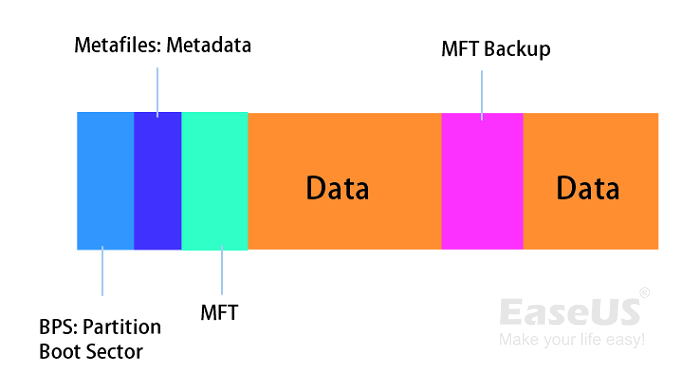
\includegraphics[width=\linewidth]{ntfs-file-system-structure.png}
\centering
\caption{Štruktúra súborového systému NTFS \\ Zdroj: https://www.easeus.com/diskmanager/file-system.html}
\end{figure}

% bulleted list plus riadkovanie iba na danu cas textu
\setstretch{1.0}
\begin{itemize}
	\item Partition Boot Sector
		\begin{itemize}
			\item Obsahuje informácie potrebné pre bootovanie. Primárne sa jedná o BootStrap čo je vlastne malý program, ktorý ma za úlohu načítať operačný systém do pamäte.
		\end{itemize}
	\item Metadata
		\begin{itemize}
			\item Pomáha definovať a organizovať súborový systém, zálohovať kritické údaje súborového systému.
		\end{itemize}
	\item Master File Table (MFT)
		\begin{itemize}
			\item Obsahuje záznamy o všetkých súboroch a adresároch na disku. Je to v podstate ekvivalent FAT tabuľky.
		\end{itemize}
	\item Data
		\begin{itemize}
			\item Obsahuje samotné dáta súborov.
		\end{itemize}
	\item MFT Backup
		\begin{itemize}
			\item Obsahuje zálohu MFT tabuľky.
		\end{itemize}
\end{itemize}




% mozem pouzit aj \ref{fig:ntfs-struct} na odkaz na obrazok

\subsubsection{Bezpečnosť NTFS}
Súborový systém NTFS umožňuje nastaviť povolenia na prístup k niektorým lokálnym súborom a priečinkom. Inými slovami, dôverný súbor môžete nastaviť tak, aby bol pre niektorých iných používateľov nedostupný.

% Mozno este toto pridat
% Pouziva ACL encryption a podobne


\subsubsection{Výhody a nevýhody NTFS}
% vytvor tabulku pre vyhody a nevyhody
\begin{table}[H]
\begin{tabularx}{\linewidth}{|X|X|}
\hline
\multicolumn{1}{|c|}{\textbf{Výhody}} & \multicolumn{1}{c|}{\textbf{Nevýhody}} \\ \hline
Podporuje veľmi veľké súbory a nemá takmer žiadne reálne obmedzenie veľkosti oddielu. & Má uzatvorený zdrojový kód. \\ \hline
Poskytuje vylepšené zabezpečenie údajov pomocou funkcií riadenia úrovne prístupu a natívneho šifrovania. & Mac OS dokáže čítať jednotky naformátované v systéme NTFS, ale na systém NTFS je možné zapisovať iba prostredníctvom softvéru tretej strany. \\ \hline
Podporuje automatickú kompresiu súborov, čo umožňuje rýchlejší prenos súborov a väčší úložný priestor na disku. & Prenosné zariadenia, ako sú smartfóny so systémom Android a digitálne fotoaparáty, ho nepodporujú. \\ \hline
Umožňuje diskové kvóty, ktoré firmám poskytujú väčšiu kontrolu nad úložným priestorom. & Kompatibilita so systémami založenými na GNU+Linux síce existuje ale iba kvôli vôli softvérových inžinerov urobiť ovladače vďaka reverznému inžinierstvu. \\ \hline
Umožňuje používateľom sledovať pridané, upravené alebo odstránené súbory na disku. &  \\ \hline
Zameriava na konzistenciu súborového systému, takže v prípade výpadku napájania alebo zlyhania systému môžete rýchlo obnoviť svoje údaje. &  \\ \hline
\end{tabularx}
\centering
\captionsetup{justification=centering,margin=2cm}
\caption{Výhody a nevýhody súborového systému NTFS \\ Zdroj: https://superops.com/ntfs-vs-fat32}
\end{table}



\subsection{ext}

\section{Nástroje na obnovu údajov}
\subsection{Testdisk}
\subsection{(Nejaký iný nástroj..)}

\section{Analýza nástroja na obnovu údajov - testdisk (táto sekcia tu asi nebude, keďže to už mám vyššie)}

\section{Experimentovanie s nástrojom testdisk}
\subsection{Zmazanie a obnova súborov}
\subsection{Zmazanie a obnova partície}

\section{Výsledky experimentov}

\section{Záver}
Temp citovanie vsetkych citacii na ich zobrazenie.\cite{TSDK,NTFS,NTFS2,NTFS3,NTFS4,FAT,EXT,ALLFS}


\bibliography{literatura}
\bibliographystyle{unsrtnat}
\end{document}